% Manual de Desarrollador
% Modificado por Crisostomo Barajas a partir del manual creado por Emmanuel Martinez
% Julio 2022

\documentclass[12pt,twoside,letter]{ol-softwaremanual}
\usepackage{float}
\usepackage[utf8]{inputenc}
\usepackage[a4paper,width=160mm,top=25mm,bottom=25mm]{geometry}
\usepackage[lining,tabular]{fbb} % so math uses tabular lining figures
\usepackage{graphicx}
\usepackage{enumitem}
\setlist{leftmargin=*}
\usepackage{listings}
\lstset{basicstyle=\ttfamily,frame=single,xleftmargin=3em,xrightmargin=3em}
\usepackage[os=win]{menukeys}
\renewmenumacro{\keys}[+]{shadowedroundedkeys}
\usepackage{framed}
\usepackage{etoolbox}
\AtBeginEnvironment{leftbar}{\sffamily\small}
\usepackage{array,lipsum}
\newenvironment{fulltable}[1][H]
 {\begin{table}[#1]%
  \hspace*{-\leftmarginwidth}%
  \begin{minipage}{\fullwidth}}
 {\end{minipage}\end{table}}
\usetikzlibrary{chains,arrows,shapes,positioning}
\usepackage{hyperref}
\graphicspath{{figures/}} %Setting the graphicspath
\renewcommand\abstractname{Introduction}

\usepackage[spanish]{babel}

\usepackage{multicol}

\usepackage{caption}
\usepackage[rightcaption]{sidecap}
\usepackage{subcaption}
\usepackage{wrapfig}
\usepackage{pifont}
\usepackage{fontawesome}

\usepackage{amsmath}
\usepackage{amssymb}

\usepackage{fancyhdr}

\pagestyle{fancy}
\fancyhf{}
\fancyhead[LE,RO]{{\footnotesize HDSP - UIS}}
\fancyhead[RE,LO]{{\footnotesize ReDs - Manual de Desarrollador}}
\fancyfoot[CE,CO]{\thepage}
%\fancyfoot[LE,RO]{\thepage}

\definecolor{ClearPurple}{RGB}{136, 0, 255}

\usepackage{tikz}
\newcommand*\circled[1]{\tikz[baseline=(char.base)]{
            \node[shape=circle,draw,inner sep=2pt] (char) {#1};}}

\newenvironment{Figure}
  {\par\medskip\noindent\minipage{\linewidth}}
  {\endminipage\par\medskip}
  
%\setlength{\parskip}{2em}
\setlength{\parskip}{6pt}%
\setlength{\parindent}{0pt}%
\setlength{\itemsep}{0em}

\title{\large{Manual de Desarrollo}\\ \vspace{10mm} \huge{Reconstrucción de Datos Sísmicos}\\ \vspace{5mm} \huge{ReDs}}
\author{
\includegraphics[width=14cm]{figures/all_logos3.png} \\ Emmanuel Martínez \\ Crisóstomo A. Barajas-Solano \\ Edwin Vargas}
\softwarelogo{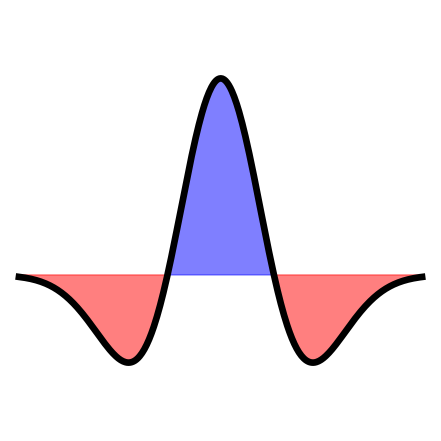
\includegraphics[width=7cm]{figures/icon}}
\version{2023.4}



\begin{document}

\maketitle

\newpage\null\thispagestyle{empty}\newpage

\begin{center}
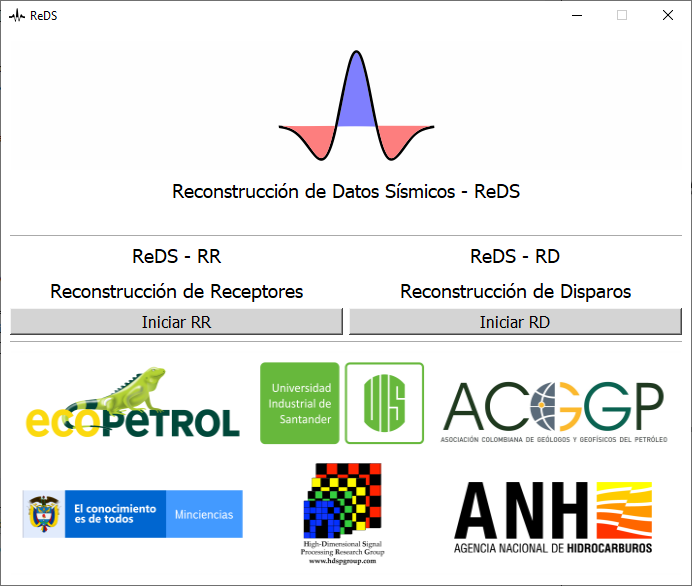
\includegraphics[width=.65\linewidth]{launch.png}
\end{center}
\begin{abstract}
%\includegraphics[width=1.0\linewidth]{PhysLogger.png}\\
%Esta aplicación pertenece al proyecto de investigación 9836, de la Universidad Industrial de Santander, Colombia. Esta aplicación permite la reconstrucción de trazas de muestras sísmicas mediante 4 diferentes algoritmos. Esta reconstrucción puede ser configurada por el usuario de tal manera que pueda realizar diferentes tipos de submuestreo y ajuste de parámetros mediante una interfaz gráfica de usuario.
La herramienta software Reconstrucción de Datos Sísmicos - ReDs hace parte del proyecto 9836 - ``Nuevas tecnologías computacionales para el diseño de sistemas de adquisición sísmica 3D terrestre con muestreo compresivo para la reducción de costos económicos e impactos ambientales en la exploración de hidrocarburos en cuencas terrestres colombianas''.

El proyecto 9836 está adscrito a la Convocatoria para la financiación de proyectos de investigación en geociencias para el sector de hidrocarburos, desarrollado por la alianza Universidad Industrial de Santander (UIS), ECOPETROL y la Asociación Colombiana de Geólogos y Geofísicos del Petróleo (ACGGP). 

Este proyecto es financiado por MINCIENCIAS y la Agencia Nacional de Hidrocarburos (ANH). Los derechos y licencias de uso sobre esta aplicación software están reservados a las entidades aportantes.
\end{abstract}

\newpage\null\thispagestyle{empty}\newpage

\clearpage
\tableofcontents

\clearpage

\newpage\null\thispagestyle{empty}\newpage

\section{Visión General de la Aplicación ReDs}

Esta aplicación Reconstrucción de Datos Sísmicos (ReDs) permite la reconstrucción de receptores y disparos sísmicos. Para esto, la aplicación ReDs dispone de dos modos de operación:
\begin{dingautolist}{192}
	\setlength\itemsep{0em}
	\item Reconstrucción de Receptores (ReDs - RR)
	\item Reconstrucción de Disparos (ReDs - RD)
\end{dingautolist}

\begin{Figure}
	\centering
	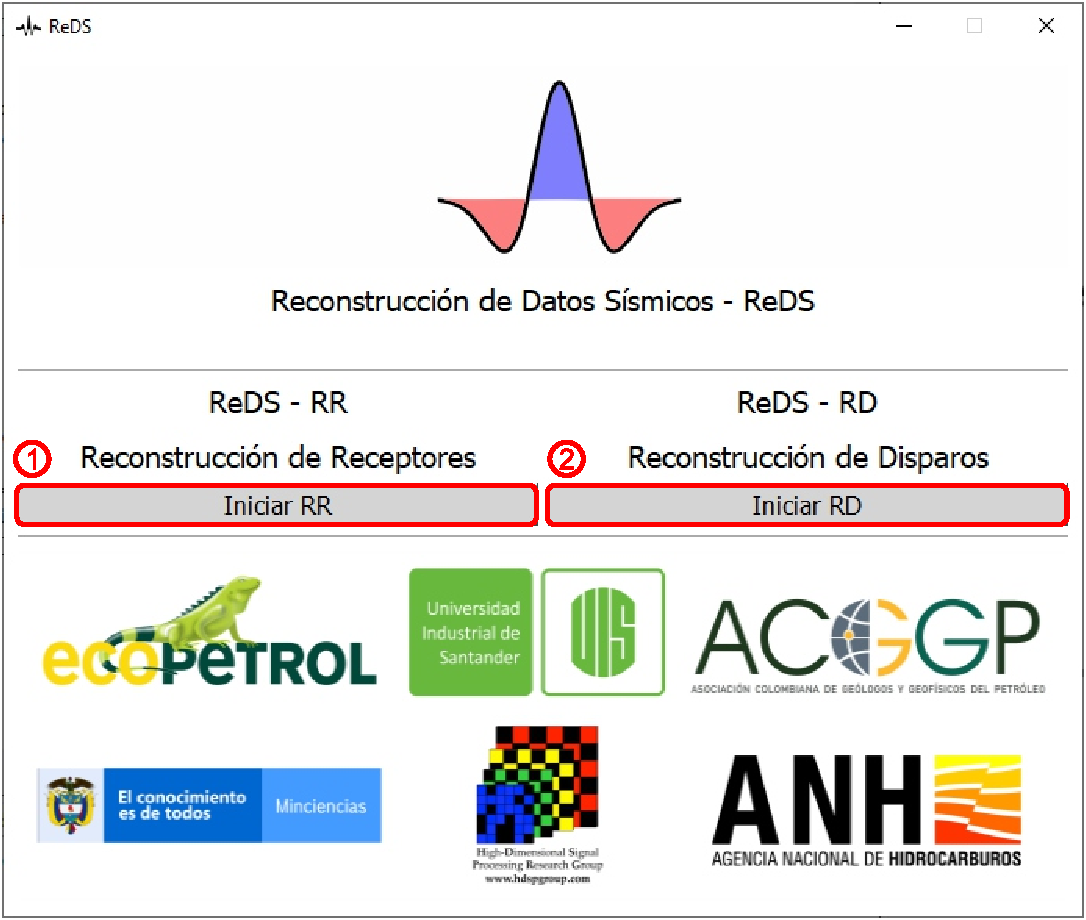
\includegraphics[width=0.65\linewidth]{launch2}
	\captionof{figure}{Secciones de la pantalla de inicio de ReDs.}
	\label{fig:launch}
\end{Figure}

Ambos modos de operación, RR y RD, realizan la reconstrucción de datos sísmicos usando 4 algoritmos numéricos diferentes:
\begin{itemize}[leftmargin=0.5in]
	\setlength\itemsep{0em}
	\item FISTA (Fast Iterative Shrinkage-Thresholding Algorithm): permite resolver problemas inversos lineales mediante un algoritmo iterativo rápido
	\item GAP (Generalized Alternating Projection): resuelve el problema de seguimiento de base grupal, que extiende el seguimiento de base reemplazando la norma $ \ell_1 $ por una norma ponderada $ \ell_{2,1} $.
	\item TwIST (Two-step Iterative Shrinkage/Thresholding): basado en el algoritmo ISTA, permite la resolución de problemas inversos
	\item ADMM (Alternating Direction Method of Multipliers): resuelve problemas de optimización convexos dividiéndolos en partes más pequeñas.
\end{itemize}

El usuario puede configurar cada uno de los algoritmos de reconstrucción de tal manera que pueda realizar diferentes tipos de submuestreo y ajuste de parámetros, todo desde una interfaz gráfica de usuario simple y clara. Aunque los modos de reconstrucción RR y RD presentan diferencias en su operación, están diseñados bajo las mismas directivas. Por esta razón, ambas interfaces gráficas cuentan con varias secciones en común.



\cleardoublepage

\section{Políticas de diseño}

La aplicación ReDs se diseñó de manera modular, la cual incluye dos módulos:

\begin{itemize}
	\item Modulo RR: Reconstrucción de Receptores
	\item Modulo RD: Reconstrucción de Disparos
\end{itemize}

Ambos módulos, a pesar de usar datos de distinta proveniencia, usan la misma lógica de diseño modular:

\begin{enumerate}
	\item Cargar datos
	\item Seleccionar rutina de reconstrucción
	\item Modificar los parámetros de la rutina de reconstrucción
	\item Seleccionar archivo de resultados
	\item Generar resultados
\end{enumerate}

Las interfaces gráficas para ambos módulos se basan en los mismos principios de uso.

\section{Diagramas UML}
A continuación se presentan los diagramas UML para el desarrollo de la aplicación ReDs.

\subsection{Diagrama de Casos de Uso Aplicación General}

El diagrama de casos de uso de la aplicación general muestra las politicas de diseño y uso generales de la aplicación ReDs. Ambos módulos se basan en el mismo diagrama, sin embargo se especializan en algunas funciones. La Figura \ref{fig:screenshot008} muestra las funcionalidades principales como:

\begin{itemize}
	\item Carga de datos
	\item Ajuste de algoritmos FISTA, ADMM, GAP, etc
	\item Ajuste de submuestreos
	\item Ajuste de experimentos
\end{itemize}

\begin{figure}
	\centering
	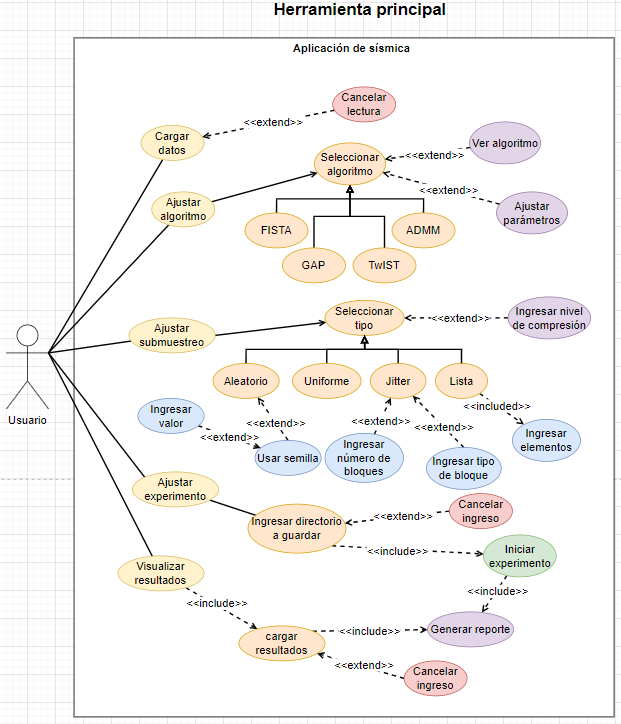
\includegraphics[width=0.7\linewidth]{figures/screenshot008}
	\caption{Diagrama de casos de uso general}
	\label{fig:screenshot008}
\end{figure}

\subsection{Diagrama de Casos de Uso Módulo RR}

La Figura \ref{fig:screenshot009} muestra en detalle los casos de uso específicos para el módulo RR.

\begin{figure}
	\centering
	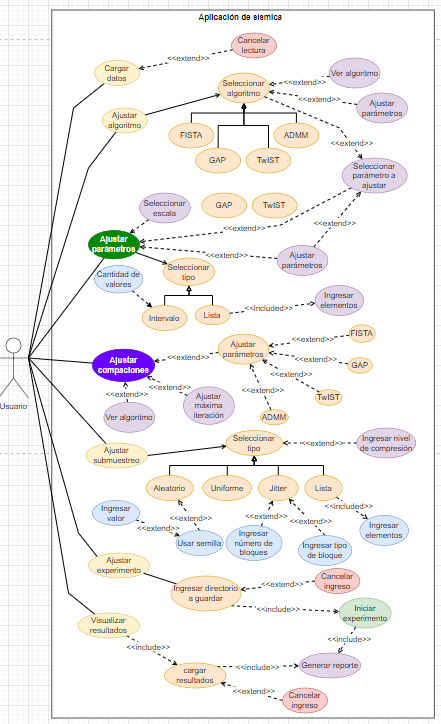
\includegraphics[width=0.7\linewidth]{figures/screenshot009}
	\caption{Diagrama de casos del módulo RR}
	\label{fig:screenshot009}
\end{figure}

\subsection{Diagrama de Casos de Uso Módulo RD}

La Figura \ref{fig:screenshot009} muestra en detalle los casos de uso específicos para el módulo RD.

\begin{figure}
	\centering
	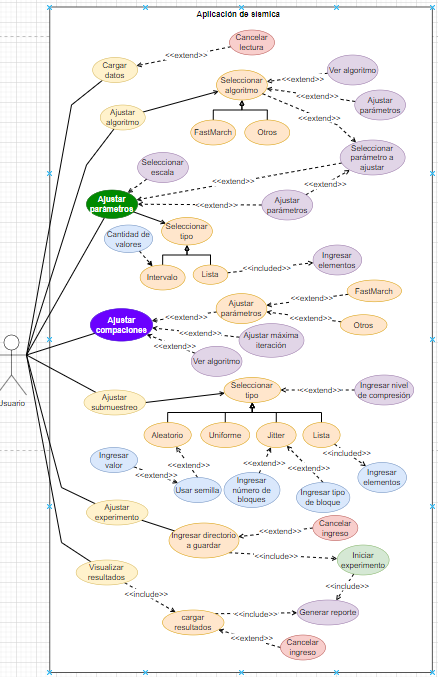
\includegraphics[width=0.7\linewidth]{figures/screenshot010}
	\caption{Diagrama de casos del módulo RD}
	\label{fig:screenshot010}
\end{figure}


\subsection{Diagrama de Secuencia Para Carga de Datos}

Para cargar los datos a procesar el usuario debe seleccionar, a través de una API del sistema operativo, la localización en disco de los archivos .dat correctamente formateados. La aplicación entonces validará o cancelará la carga del archivo .dat escogido. Ver Figura \ref{fig:screenshot001}.

\begin{figure}
	\centering
	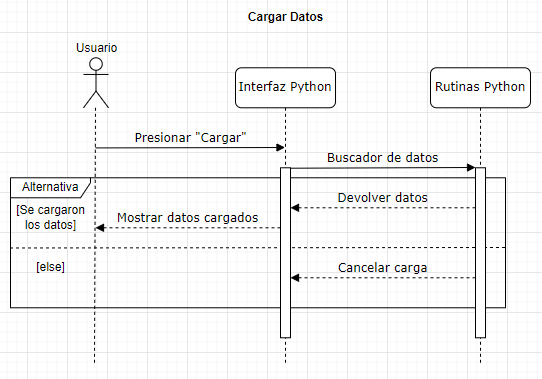
\includegraphics[width=0.7\linewidth]{figures/screenshot001}
	\caption{Diagrama de Secuencia para cargar datos}
	\label{fig:screenshot001}
\end{figure}

\subsection{Diagrama de Secuencia para Guardar Experimento}

Antes de iniciar cualquier experimento es necesario seleccionar el archivo destino de los resultados del experimento. Esto se hace a través del API del sistema. Ver Figura \ref{fig:screenshot002}.

\begin{figure}
	\centering
	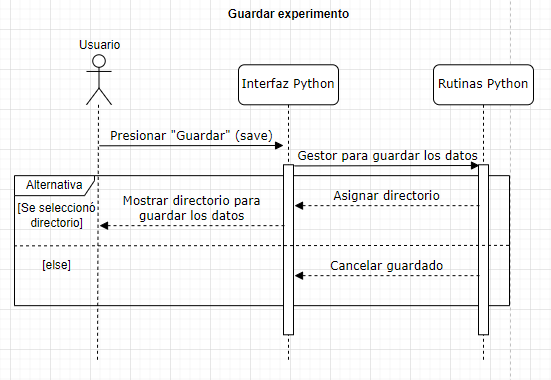
\includegraphics[width=0.7\linewidth]{figures/screenshot002}
	\caption{Diagrama de Secuencia para guardar experimento}
	\label{fig:screenshot002}
\end{figure}

\subsection{Diagrama de Secuencia para Ajuste de Algoritmo}

Cada rutina de reconstrucción puede ser ajustada manualmente usando la interfaz de usuario. Ver Figura \ref{fig:screenshot005}.

\begin{figure}
	\centering
	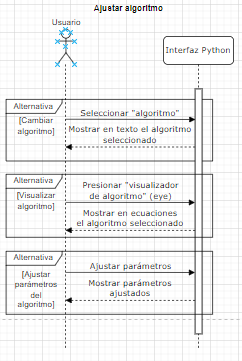
\includegraphics[width=0.4\linewidth]{figures/screenshot005}
	\caption{Diagrama de Secuencia para ajuste de algoritmo}
	\label{fig:screenshot005}
\end{figure}

\subsection{Diagrama de Secuencia de Inicio de Experimentos}

Una vez se ha seleccionado el archivo de datos, el ajuste del algoritmo y la selección del archivo de resultados, se puede dar paso a la realización del experimento. Ver Figura \ref{fig:screenshot006}.

\begin{figure}
	\centering
	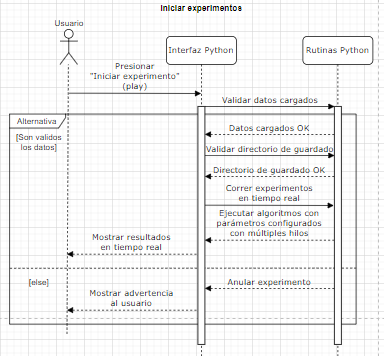
\includegraphics[width=0.7\linewidth]{figures/screenshot006}
	\caption{Diagrama de Secuencia para inicio de experimento}
	\label{fig:screenshot006}
\end{figure}


\subsection{Diagrama de Secuencia para Ajuste de Parámetros}

El usuario puede realizar un ajuste de parámetros para una rutina de reconstrucción específica. Esta se puede realizar dentro de un intervalo, un cambio de escala o introduciendo valores específicos. Ver Figura \ref{fig:screenshot003}.

\begin{figure}
	\centering
	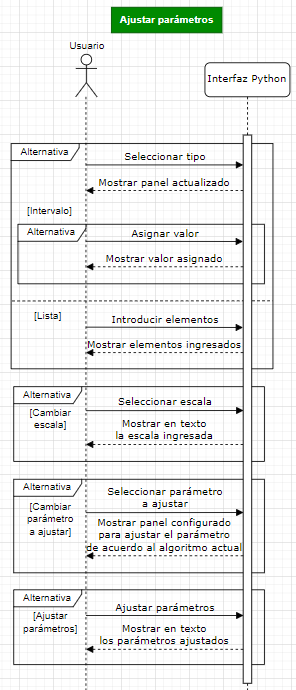
\includegraphics[width=0.48\linewidth]{figures/screenshot003}
	\caption{Diagrama de Secuencia para ajuste de parámetros}
	\label{fig:screenshot003}
\end{figure}

\subsection{Diagrama de Secuencia para Ajuste de Comparaciones}

Una vez realizadas el ajuste de parámetros para una rutina en específico, se puede realizar la comparación entre varias rutinas de reconstrucción. Para esto se debe realizar la misma selección de ajuste de parámetros para cada rutina, individualmente, y luego proceder a realizar el ajuste colectivo. Ver Figura \ref{fig:screenshot004}.

\begin{figure}
	\centering
	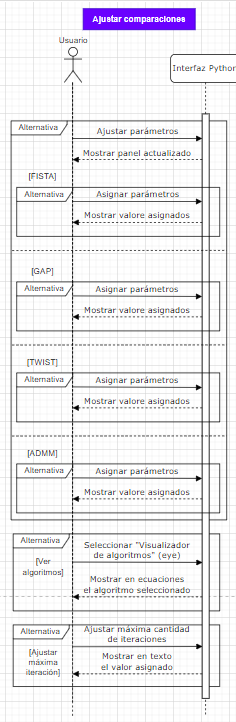
\includegraphics[width=0.4\linewidth]{figures/screenshot004}
	\caption{Diagrama de Secuencia para ajuste de comparaciones}
	\label{fig:screenshot004}
\end{figure}




\end{document}